\documentclass{article}\usepackage[]{graphicx}\usepackage[]{color}
%% maxwidth is the original width if it is less than linewidth
%% otherwise use linewidth (to make sure the graphics do not exceed the margin)
\makeatletter
\def\maxwidth{ %
  \ifdim\Gin@nat@width>\linewidth
    \linewidth
  \else
    \Gin@nat@width
  \fi
}
\makeatother

\definecolor{fgcolor}{rgb}{0.345, 0.345, 0.345}
\newcommand{\hlnum}[1]{\textcolor[rgb]{0.686,0.059,0.569}{#1}}%
\newcommand{\hlstr}[1]{\textcolor[rgb]{0.192,0.494,0.8}{#1}}%
\newcommand{\hlcom}[1]{\textcolor[rgb]{0.678,0.584,0.686}{\textit{#1}}}%
\newcommand{\hlopt}[1]{\textcolor[rgb]{0,0,0}{#1}}%
\newcommand{\hlstd}[1]{\textcolor[rgb]{0.345,0.345,0.345}{#1}}%
\newcommand{\hlkwa}[1]{\textcolor[rgb]{0.161,0.373,0.58}{\textbf{#1}}}%
\newcommand{\hlkwb}[1]{\textcolor[rgb]{0.69,0.353,0.396}{#1}}%
\newcommand{\hlkwc}[1]{\textcolor[rgb]{0.333,0.667,0.333}{#1}}%
\newcommand{\hlkwd}[1]{\textcolor[rgb]{0.737,0.353,0.396}{\textbf{#1}}}%
\let\hlipl\hlkwb

\usepackage{framed}
\makeatletter
\newenvironment{kframe}{%
 \def\at@end@of@kframe{}%
 \ifinner\ifhmode%
  \def\at@end@of@kframe{\end{minipage}}%
  \begin{minipage}{\columnwidth}%
 \fi\fi%
 \def\FrameCommand##1{\hskip\@totalleftmargin \hskip-\fboxsep
 \colorbox{shadecolor}{##1}\hskip-\fboxsep
     % There is no \\@totalrightmargin, so:
     \hskip-\linewidth \hskip-\@totalleftmargin \hskip\columnwidth}%
 \MakeFramed {\advance\hsize-\width
   \@totalleftmargin\z@ \linewidth\hsize
   \@setminipage}}%
 {\par\unskip\endMakeFramed%
 \at@end@of@kframe}
\makeatother

\definecolor{shadecolor}{rgb}{.97, .97, .97}
\definecolor{messagecolor}{rgb}{0, 0, 0}
\definecolor{warningcolor}{rgb}{1, 0, 1}
\definecolor{errorcolor}{rgb}{1, 0, 0}
\newenvironment{knitrout}{}{} % an empty environment to be redefined in TeX

\usepackage{alltt}
\usepackage{natbib}



\IfFileExists{upquote.sty}{\usepackage{upquote}}{}
\begin{document}

\title{Wuthering Heights Wordcoud}
\author{Madam President Cake AKA Heidi L Beezub}
\maketitle

\begin{abstract}
This paper provides the steps to create a wordcloud with R-studio using a work that is part of the Project Gutenberg collection which makes classic texts available for free.  In addition, it includes the steps involved in creating a latex document (what you are reading).

\end{abstract}

\section{Preparing R-Studio}
In order to create our word cloud in R-Studio we first have to install the various packages we'll use to extract the data, create our word cloud and then to format everything into our latex document.
We'll need to install the following packages: dplyr, tidytext, stringr, wordcloud, tm, gutenbergr, and knitr.  If you already have the packages installed, you can skip to the next step and library each package into R-Studio.  Once you have all the packages installed and library-ed, open a new R script file. 

\section{Finding our text}
We will be using the gutenbergr package to retrieve a text.  The gutenbergr package allows us to download and process public domain works in the Project Gutenberg collection. Includes metadata for all Project Gutenberg works, so that they can be searched and retrieved. \footnote{https://cran.r-project.org/web/packages/gutenbergr/index.html}  We'll be looking for Wuthering Heights by Emily Bronte.  

The following code also uses stringr so that we don't have to have the information exactly as it is the data.  We will need to add the libraries for stringr \& gutenbergr to our code so that it will run.

\begin{knitrout}
\definecolor{shadecolor}{rgb}{0.969, 0.969, 0.969}\color{fgcolor}\begin{kframe}
\begin{alltt}
\hlkwd{library}\hlstd{(stringr)}
\hlkwd{library}\hlstd{(gutenbergr)}
\hlkwd{library}\hlstd{(dplyr)}
\end{alltt}


{\ttfamily\noindent\itshape\color{messagecolor}{\#\# \\\#\# Attaching package: 'dplyr'}}

{\ttfamily\noindent\itshape\color{messagecolor}{\#\# The following objects are masked from 'package:stats':\\\#\# \\\#\#\ \ \ \  filter, lag}}

{\ttfamily\noindent\itshape\color{messagecolor}{\#\# The following objects are masked from 'package:base':\\\#\# \\\#\#\ \ \ \  intersect, setdiff, setequal, union}}\begin{alltt}
\hlkwd{gutenberg_works}\hlstd{(}\hlkwd{str_detect}\hlstd{(author,} \hlstr{"Bront�"}\hlstd{))}
\end{alltt}
\begin{verbatim}
## # A tibble: 8 x 8
##   gutenberg_id                       title            author
##          <int>                       <chr>             <chr>
## 1          767                  Agnes Grey      Bront�, Anne
## 2          768           Wuthering Heights     Bront�, Emily
## 3          969 The Tenant of Wildfell Hall      Bront�, Anne
## 4         1028               The Professor Bront�, Charlotte
## 5         1260 Jane Eyre: An Autobiography Bront�, Charlotte
## 6         9182                    Villette Bront�, Charlotte
## 7        17081               Cottage Poems   Bront�, Patrick
## 8        30486                     Shirley Bront�, Charlotte
## # ... with 5 more variables: gutenberg_author_id <int>, language <chr>,
## #   gutenberg_bookshelf <chr>, rights <chr>, has_text <lgl>
\end{verbatim}
\end{kframe}
\end{knitrout}

We've got more than one text listed so we'll need to refine our search:

\begin{knitrout}
\definecolor{shadecolor}{rgb}{0.969, 0.969, 0.969}\color{fgcolor}\begin{kframe}
\begin{alltt}
\hlkwd{gutenberg_works}\hlstd{(author} \hlopt{==} \hlstr{"Bront�, Emily"}\hlstd{,}\hlkwd{str_detect}\hlstd{(title,} \hlstr{"Wuthering"}\hlstd{))}
\end{alltt}
\begin{verbatim}
## # A tibble: 1 x 8
##   gutenberg_id             title        author gutenberg_author_id
##          <int>             <chr>         <chr>               <int>
## 1          768 Wuthering Heights Bront�, Emily                 405
## # ... with 4 more variables: language <chr>, gutenberg_bookshelf <chr>,
## #   rights <chr>, has_text <lgl>
\end{verbatim}
\end{kframe}
\end{knitrout}

The number `768' is the Gutenberg identification number or gutenberg\_id.  We'll use this number to download our text.
\begin{knitrout}
\definecolor{shadecolor}{rgb}{0.969, 0.969, 0.969}\color{fgcolor}\begin{kframe}
\begin{alltt}
\hlkwd{gutenberg_download}\hlstd{(}\hlnum{768}\hlstd{)}
\end{alltt}


{\ttfamily\noindent\itshape\color{messagecolor}{\#\# Determining mirror for Project Gutenberg from http://www.gutenberg.org/robot/harvest}}

{\ttfamily\noindent\itshape\color{messagecolor}{\#\# Using mirror http://aleph.gutenberg.org}}\begin{verbatim}
## # A tibble: 12,085 x 2
##    gutenberg_id
##           <int>
##  1          768
##  2          768
##  3          768
##  4          768
##  5          768
##  6          768
##  7          768
##  8          768
##  9          768
## 10          768
## # ... with 12,075 more rows, and 1 more variables: text <chr>
\end{verbatim}
\end{kframe}
\end{knitrout}

Now that we have the right book, we'll save this into our data frame variable wh. 

\begin{knitrout}
\definecolor{shadecolor}{rgb}{0.969, 0.969, 0.969}\color{fgcolor}\begin{kframe}
\begin{alltt}
\hlstd{wh} \hlkwb{<-} \hlkwd{gutenberg_download}\hlstd{(}\hlnum{768}\hlstd{)}
\end{alltt}
\end{kframe}
\end{knitrout}

Now we'll take a quick look at our data by looking at the head (first rows):

\begin{knitrout}
\definecolor{shadecolor}{rgb}{0.969, 0.969, 0.969}\color{fgcolor}\begin{kframe}
\begin{alltt}
\hlkwd{head}\hlstd{(wh)}
\end{alltt}
\begin{verbatim}
## # A tibble: 6 x 2
##   gutenberg_id              text
##          <int>             <chr>
## 1          768 WUTHERING HEIGHTS
## 2          768                  
## 3          768                  
## 4          768         CHAPTER I
## 5          768                  
## 6          768
\end{verbatim}
\end{kframe}
\end{knitrout}

It looks like the data loaded into our wh variable.

Even though we don't have to, let's get rid of the words `chapter.'

\begin{knitrout}
\definecolor{shadecolor}{rgb}{0.969, 0.969, 0.969}\color{fgcolor}\begin{kframe}
\begin{alltt}
\hlkwd{library}\hlstd{(tidytext)}
\hlkwd{library}\hlstd{(tm)}
\end{alltt}


{\ttfamily\noindent\itshape\color{messagecolor}{\#\# Loading required package: NLP}}\begin{alltt}
\hlstd{wh}\hlopt
  \hlkwd{filter}\hlstd{(}\hlopt{!}\hlkwd{str_detect}\hlstd{(wh}\hlopt{$}\hlstd{text,}\hlstr{'^CHAPTER'}\hlstd{))}
\end{alltt}
\begin{verbatim}
## # A tibble: 12,051 x 2
##    gutenberg_id
##           <int>
##  1          768
##  2          768
##  3          768
##  4          768
##  5          768
##  6          768
##  7          768
##  8          768
##  9          768
## 10          768
## # ... with 12,041 more rows, and 1 more variables: text <chr>
\end{verbatim}
\end{kframe}
\end{knitrout}

We can see in the R-studio console that the word chapter (that we could see before in line 3 has been removed. We'll save this into our wh data frame variable  

\begin{knitrout}
\definecolor{shadecolor}{rgb}{0.969, 0.969, 0.969}\color{fgcolor}\begin{kframe}
\begin{alltt}
\hlstd{wh}\hlkwb{<-}\hlstd{wh}\hlopt
  \hlkwd{filter}\hlstd{(}\hlopt{!}\hlkwd{str_detect}\hlstd{(wh}\hlopt{$}\hlstd{text,}\hlstr{'^CHAPTER'}\hlstd{))}
\hlkwd{head}\hlstd{(wh)}
\end{alltt}
\begin{verbatim}
## # A tibble: 6 x 2
##   gutenberg_id
##          <int>
## 1          768
## 2          768
## 3          768
## 4          768
## 5          768
## 6          768
## # ... with 1 more variables: text <chr>
\end{verbatim}
\end{kframe}
\end{knitrout}

We can also see that lines 1-5 only contain the title \& all the rest are blank lines.  Let's get rid of these as well.  The wh[1:6,] is calling the row numbers 1 to 6.  The space after the comma would be if we wanted to limit the rows.
\begin{knitrout}
\definecolor{shadecolor}{rgb}{0.969, 0.969, 0.969}\color{fgcolor}\begin{kframe}
\begin{alltt}
\hlstd{wh[}\hlnum{1}\hlopt{:}\hlnum{6}\hlstd{,]}
\end{alltt}
\begin{verbatim}
## # A tibble: 6 x 2
##   gutenberg_id
##          <int>
## 1          768
## 2          768
## 3          768
## 4          768
## 5          768
## 6          768
## # ... with 1 more variables: text <chr>
\end{verbatim}
\end{kframe}
\end{knitrout}

We'll need to know the total number of lines so let's get the dimensions of our data frame:
\begin{knitrout}
\definecolor{shadecolor}{rgb}{0.969, 0.969, 0.969}\color{fgcolor}\begin{kframe}
\begin{alltt}
\hlkwd{dim}\hlstd{(wh)}
\end{alltt}
\begin{verbatim}
## [1] 12051     2
\end{verbatim}
\end{kframe}
\end{knitrout}

So now that we know our dimensions, we'll save only the line numbers we want to keep into our wh data frame variable. Again, since there is nothing after the comma we aren't limiting any columns.

\begin{knitrout}
\definecolor{shadecolor}{rgb}{0.969, 0.969, 0.969}\color{fgcolor}\begin{kframe}
\begin{alltt}
\hlstd{wh}\hlkwb{<-}\hlstd{wh[}\hlnum{6}\hlopt{:}\hlnum{12051}\hlstd{,]}
\end{alltt}
\end{kframe}
\end{knitrout}

Now when we call the wh variable, we see that all the blank lines are gone.  Note that the lines are re-numbered as well.Again, we can see this in the R-studio console.
\begin{knitrout}
\definecolor{shadecolor}{rgb}{0.969, 0.969, 0.969}\color{fgcolor}\begin{kframe}
\begin{alltt}
\hlstd{wh}
\end{alltt}
\begin{verbatim}
## # A tibble: 12,046 x 2
##    gutenberg_id
##           <int>
##  1          768
##  2          768
##  3          768
##  4          768
##  5          768
##  6          768
##  7          768
##  8          768
##  9          768
## 10          768
## # ... with 12,036 more rows, and 1 more variables: text <chr>
\end{verbatim}
\end{kframe}
\end{knitrout}


Now we want to break the lines of text into individual words.  We use the unnest function from tidytext.  The unnest needs (input, output).  For our output (which we'll call word) it will make a column called `word'.  The input (which we'll call text) will be the individual words.

\begin{knitrout}
\definecolor{shadecolor}{rgb}{0.969, 0.969, 0.969}\color{fgcolor}\begin{kframe}
\begin{alltt}
\hlstd{wh}\hlopt
  \hlkwd{filter}\hlstd{(}\hlopt{!}\hlkwd{str_detect}\hlstd{(wh}\hlopt{$}\hlstd{text,}\hlstr{'^CHAPTER'}\hlstd{))}
\end{alltt}
\begin{verbatim}
## # A tibble: 12,046 x 2
##    gutenberg_id
##           <int>
##  1          768
##  2          768
##  3          768
##  4          768
##  5          768
##  6          768
##  7          768
##  8          768
##  9          768
## 10          768
## # ... with 12,036 more rows, and 1 more variables: text <chr>
\end{verbatim}
\end{kframe}
\end{knitrout}
We can see in the R-studio console that the word chapter (that we could see before in line 3 has been removed).
(Again) we'll save this back into a new variable words\_wh.
\begin{knitrout}
\definecolor{shadecolor}{rgb}{0.969, 0.969, 0.969}\color{fgcolor}\begin{kframe}
\begin{alltt}
\hlstd{wh}\hlkwb{<-}\hlstd{wh}\hlopt
  \hlkwd{filter}\hlstd{(}\hlopt{!}\hlkwd{str_detect}\hlstd{(wh}\hlopt{$}\hlstd{text,}\hlstr{'^CHAPTER'}\hlstd{))}
\end{alltt}
\end{kframe}
\end{knitrout}

Now we want to break the lines of text into individual words.  We use the unnest function from tidytext.  We'll bring in the library for tidy text and tm (text mining) .  The unnest needs (input, output).  For our output (which we'll call word) it will make a column called `word'.  The input (which we'll call text) will be the individual words.

\begin{knitrout}
\definecolor{shadecolor}{rgb}{0.969, 0.969, 0.969}\color{fgcolor}\begin{kframe}
\begin{alltt}
\hlstd{wh}\hlopt
  \hlkwd{unnest_tokens}\hlstd{(word,text)}
\end{alltt}
\begin{verbatim}
## # A tibble: 117,041 x 2
##    gutenberg_id     word
##           <int>    <chr>
##  1          768     1801
##  2          768        i
##  3          768     have
##  4          768     just
##  5          768 returned
##  6          768     from
##  7          768        a
##  8          768    visit
##  9          768       to
## 10          768       my
## # ... with 117,031 more rows
\end{verbatim}
\end{kframe}
\end{knitrout}
We'll save this back into a new variable called words\_wh

\begin{knitrout}
\definecolor{shadecolor}{rgb}{0.969, 0.969, 0.969}\color{fgcolor}\begin{kframe}
\begin{alltt}
\hlstd{words_wh} \hlkwb{<-} \hlstd{wh}\hlopt
  \hlkwd{unnest_tokens}\hlstd{(word,text)}
\end{alltt}
\end{kframe}
\end{knitrout}
head(wh\$text)

\section{Stop Words}
Now that we have the individual words we just need a couple more steps before we can make our word cloud.  We want to get rid of all the `stop words.'  These are the 'small' words like in, the, a, an, at , to, etc.The 'list' of stop wprds is part of the tidytext package.
\begin{knitrout}
\definecolor{shadecolor}{rgb}{0.969, 0.969, 0.969}\color{fgcolor}\begin{kframe}
\begin{alltt}
\hlstd{words_wh}\hlopt
  \hlkwd{filter}\hlstd{(}\hlopt{!}\hlstd{(word} \hlopt \hlstd{stop_words}\hlopt{$}\hlstd{word))}
\end{alltt}
\begin{verbatim}
## # A tibble: 40,503 x 2
##    gutenberg_id      word
##           <int>     <chr>
##  1          768      1801
##  2          768  returned
##  3          768     visit
##  4          768  landlord
##  5          768  solitary
##  6          768 neighbour
##  7          768  troubled
##  8          768 beautiful
##  9          768   country
## 10          768   england
## # ... with 40,493 more rows
\end{verbatim}
\end{kframe}
\end{knitrout}

Again, we'll save these all back into our variable words\_wh:
\begin{knitrout}
\definecolor{shadecolor}{rgb}{0.969, 0.969, 0.969}\color{fgcolor}\begin{kframe}
\begin{alltt}
\hlstd{words_wh}\hlkwb{<-}\hlstd{words_wh}\hlopt
  \hlkwd{filter}\hlstd{(}\hlopt{!}\hlstd{(word} \hlopt \hlstd{stop_words}\hlopt{$}\hlstd{word))}
\end{alltt}
\end{kframe}
\end{knitrout}

\section{Getting Ready for Our Wordcloud}
Now that we only the `main' or important words, we'll group these words together to get the frequency of each word.

\begin{knitrout}
\definecolor{shadecolor}{rgb}{0.969, 0.969, 0.969}\color{fgcolor}\begin{kframe}
\begin{alltt}
\hlstd{words_wh}\hlopt
  \hlkwd{group_by}\hlstd{(word)}\hlopt
  \hlkwd{summarise}\hlstd{(}\hlkwc{count}\hlstd{=}\hlkwd{n}\hlstd{())}
\end{alltt}
\begin{verbatim}
## # A tibble: 8,875 x 2
##         word count
##        <chr> <int>
##  1     _all_     1
##  2  _almost_     2
##  3      _am_     2
##  4 _anybody_     1
##  5     _are_     4
##  6      _bed     2
##  7  _better_     1
##  8   _books_     2
##  9     _can_     1
## 10  _cannot_     2
## # ... with 8,865 more rows
\end{verbatim}
\end{kframe}
\end{knitrout}

We'll save this into a variable word\_freq\_wh:

\begin{knitrout}
\definecolor{shadecolor}{rgb}{0.969, 0.969, 0.969}\color{fgcolor}\begin{kframe}
\begin{alltt}
\hlstd{word_freq_wh}\hlkwb{<-}\hlstd{words_wh}\hlopt
  \hlkwd{group_by}\hlstd{(word)}\hlopt
  \hlkwd{summarise}\hlstd{(}\hlkwc{count}\hlstd{=}\hlkwd{n}\hlstd{())}
\end{alltt}
\end{kframe}
\end{knitrout}

\section{Wordcloud}
Now we are ready for our wordcloud. We'll need to bring in the wordcloud library.  The minimum frequency number helps to determine the size.  If we use a larger number (like 50 or 100) it makes our word cloud smaller (less words).  A smaller number gives us more words, but many of the words are smaller.  Basically we need to 'play' with the min.freq number until we get something that looks appealing.  
\begin{knitrout}
\definecolor{shadecolor}{rgb}{0.969, 0.969, 0.969}\color{fgcolor}\begin{kframe}
\begin{alltt}
\hlkwd{library}\hlstd{(wordcloud)}
\end{alltt}


{\ttfamily\noindent\itshape\color{messagecolor}{\#\# Loading required package: RColorBrewer}}\begin{alltt}
\hlkwd{wordcloud}\hlstd{(word_freq_wh}\hlopt{$}\hlstd{word,word_freq_wh}\hlopt{$}\hlstd{count,}\hlkwc{min.freq}\hlstd{=}\hlnum{25}\hlstd{)}
\end{alltt}
\end{kframe}
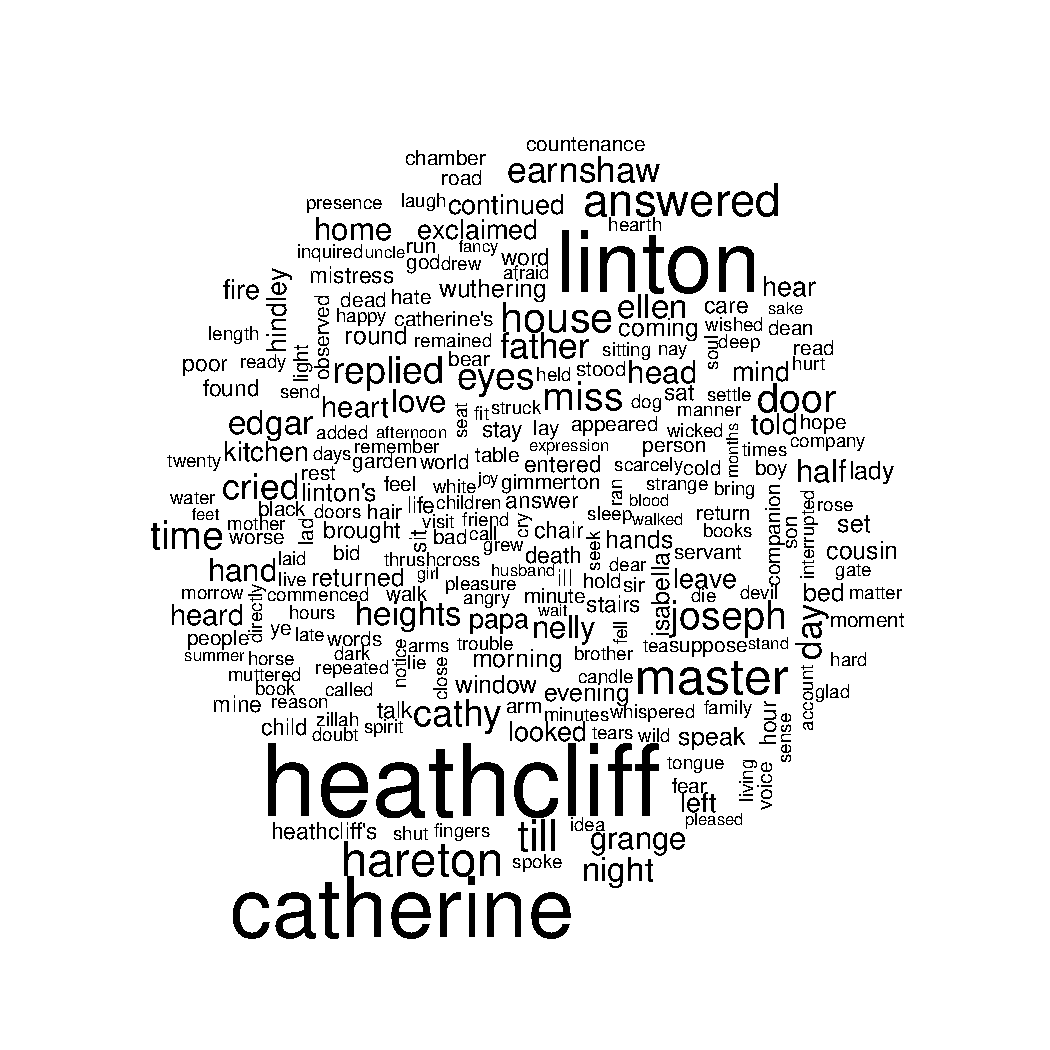
\includegraphics[width=\maxwidth]{figure/unnamed-chunk-21-1} 

\end{knitrout}

Looks pretty good, but let's see if we can add some color.

\begin{knitrout}
\definecolor{shadecolor}{rgb}{0.969, 0.969, 0.969}\color{fgcolor}\begin{kframe}
\begin{alltt}
\hlkwd{wordcloud}\hlstd{(word_freq_wh}\hlopt{$}\hlstd{word,word_freq_wh}\hlopt{$}\hlstd{count,}\hlkwc{min.freq}\hlstd{=}\hlnum{35}\hlstd{,}\hlkwc{colors}\hlstd{=}\hlkwd{brewer.pal}\hlstd{(}\hlnum{5}\hlstd{,}\hlstr{'Dark2'}\hlstd{))}
\end{alltt}
\end{kframe}
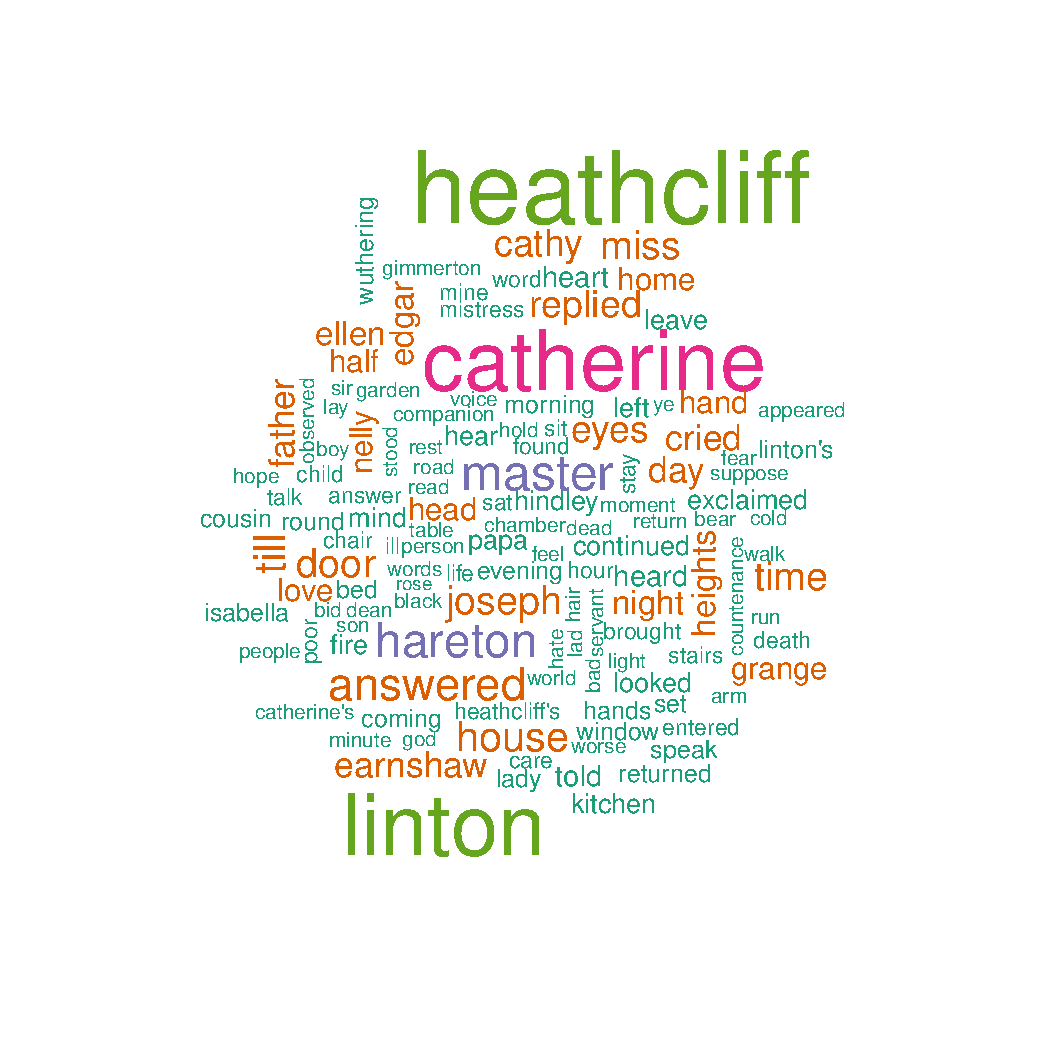
\includegraphics[width=\maxwidth]{figure/unnamed-chunk-22-1} 

\end{knitrout}

\section{Latex Document how to}
First under Tools then Global Options  choose Sweve on the left \& at the top change Sweave to Kntr

Now open a new Sweave file.
It opens up showing:
backslash documentclass\{article\}

backslash begin\{document\}

backslash end\{document\}
These control the Sweave document.  If the Begin or end document aren't paired, it will not compile into a pdf.  MAKE SURE that the backslash end document is always the last thing.  Put several returns before it to make sure you have "room" to work \& keep this at the bottom of the page.

After the begin document type in the following:

backslash title\{wordcoud\}
backslash author{Madam President Cake AKA Heidi L Beezub\}
backslash maketitle

Then we need to add
backslash begin\{abstract\}

backslsh character end\{abstract\}
You need to thave the corresponding "end"   Type the summary intro for our paper between the beginning \& end.

Take note.  Sweave uses special characters.  For example if you type an ampersand \& you have to use a backslash \ in front of it, or Sweave wants to read it as a function.

The backslash \ is the escape character (double backslash can be used to create a new line).\\
A backslash needs to go before the underscore \_ or ampersand \& as these have special meaning in R for formatting text.\\
The right carrot I gather is for a new paragraph but you can't use the escape backslash to escape out of it.
Use the tic mark in upper left key (under the tilde) for the first quote and the last quote is the regular quote mark. If using double quotes you need 2 tics.  Note that for a contraction such as can't you use the regular quote mark.

As we put in each section of the Sweave, be sure to hit the 'Compile Pdf' button.  That way you will know your document is compiling.

If you get an error message it will have a line number (that doesn't correspond to your Sweave document line numbers).  Go to the 'view log' button  (just above the error messages).  Scroll through until you see a (what looks like a number 1 but is really an l) 
It gives you the "text" where you made the mistake you just need to find it \& fix it.

Now we are ready to add a section.  We type
backslash section\{Section Title\}
With the section title in between the curley brackets \{\}
Sweave keeps track of the section numbers \& if we add a section in the middle it automatically re-numbers.

We can type text (keeping in mind those special characters)
And insert r code using the green `+c' icon at the top right of the working sweave file.

When we compile the pdf, it shows not only the code, but the code output.

We added text \& code based on our data.

\section{Latex Bibliography}

For our bibliography we have to do several things.

At the top of our document right under the document class we need to add
Backslash usepackage\{natbib\}
Directly under that we need to add the following code:

because of all the special characters it is best to look at a sample document \& copy or modify the text to fit your needs.
Left carrot left carrot echo equal sign FALSE right carrot right carrot equal sign
Packages left carrot dash c(`dplyr',`stringr',`tidytext',`wordcloud',`tm',`janeaustenr')
knitr colon colon write\_bib(packages,file equal sign 'packages.bib')
/@

Then just before the end document  put in:
Backslash bibliographystyle\{apa\}
Backslash bibliography\{Wordcloud\_WutheringHeights,packages\}
Backslash nocite\{\*\}

Open a new text file in R \& save as the same name as your document but with an extension of .bib.
Look at an example for the required format

THEN go to the terminal. Make sure the director is correct for the folder you are working on.
type inthe following in this order \& let each run:

pdflatex Wordcloud\_WutheringHeights
bibtex Wordcloud\_WutheringHeights
pdflatex Wordcloud\_WutheringHeights
pdflatex Wordcloud\_WutheringHeights

you will get veriage afeter each so you know that it has been accepted and processed.

If your bibliography compiles and then won't later on, go into the folder \& delete all the system created folders and try the pdf latex in the terminal again.

\bibliographystyle{apa}
\bibliography{Wordcloud_WutheringHeights,packages}
\nocite{*}


\end{document}
